\icode{E-MD-SI-L2-261115-003}
如图所示，$A$、$B$两球用细线悬挂于天花板上且静止不动，两球质量 $m_A = 2m_B$，两球间是一个轻质弹簧，如果突然剪断悬线，则在剪断悬线瞬间\paren[]
	
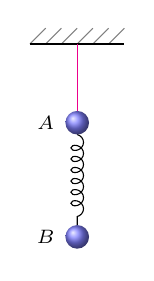
\begin{tikzpicture}[font=\scriptsize]
	\foreach \x in {-.6,-.4,...,.6}
			\draw[gray] (\x,0)--++(.2,.2);
	\draw[thick] (-.6,0)--(.6,0);
	\draw[decoration={aspect=.8,segment length=4,amplitude=.8mm,coil},decorate] (0,-1.15)--(0,-2.3);
	\draw[magenta] (0,0)--(0,-1);
	\shade[ball color=blue!50] (0,-1) circle(.15);
	\shade[ball color=blue!50] (0,-2.45) circle(.15);
	\node at(-.4,-1){\(A\)};
	\node at(-.4,-2.45){\(B\)};
\end{tikzpicture}
\begin{choices}
	\item $A$球加速度为 $\frac{3}{2} g$，$B$球加速度为\(g\)
	\item $A$球加速度为 $\frac{3}{2} g$，$B$球加速度为0
	\item $A$球加速度为 $\frac{1}{2} g$，$B$球加速度为0
	\item $A$球加速度为 $\frac{1}{2} g$，$B$球加速度为\(g\)
\end{choices}
\begin{answer}
    B\qquad 提示：
\end{answer}